\section{Calcul de la mesure}\label{sec:calcul_mesure}

\subsection{Ancien algorithme}
\todo{Ancien algorithme}

\subsection{Nouvel algorithme}

\todo{Le problème des calculs de chemin dans les graphes temporels}

Le problème des plus courts chemins est déjà assez complexe dans un graphe classique, mais il devient encore plus difficile dans un graphe temporel,
où les arêtes peuvent être bloquées à certains moments.
Nous sommes d'abord partis sur une adaptation de l'algorithme de Floyd-Warshall, car nous savons que cet algorithme marche tout type de graphe, 
notamment des graphes étranges comme les ceux avec des arêtes à poids négatifs.

\begin{algorithm}[H]
    TemporalFloydWarshall(graphe temporel \ GT, DistanceMatrixes \ dma)
\begin{algorithmic}
	\State $InitTFW(GT, dma)$

	\For {$time \ in \ \{dma.NumMatrixes \ .. \ 0 \} $}
		\For { $k \ in \ \{ 0 \ .. \ |GT.V| \ \} $}
			\For { $u \ in \ \{ 0 \ .. \ |GT.V| \ \} $}
				\For { $v \ in \ \{ 0 \ .. \ |GT.V| \ \} $}
				
					\State $distUV \gets dma.matrix[t_{i}][u][v]$
					\State $distUK \gets dma.matrix[t_{i}][u][k]$
					\State $distKV \gets dma.matrix[t_{i}+distUK][k][v]$

					\If{$distUV > distUK + distKV$}
						\State $dma.matrix[t_{i}][u][v] \gets distUK + distKV$
					\EndIf
				\EndFor
			\EndFor
		\EndFor
	\EndFor 
\end{algorithmic}
\end{algorithm}

\subsubsection{Création d'une structure de données adaptée}
Le problème des autres algorithmes classiques de graphes est qu'ils ne peuvent pas voir dans le futur, et donc ne peuvent pas prendre en compte les liens bloqués.
Cependannt, nous avons pensé à créer des liens fantômes qui remplacent les liens supprimés, équivalents à la distance réelle plus l'attente nécessaire.
Cela va permettre de ne pas avoir besoin de regarder dans le futur pour calculer les chemins, tout en calculant quand même la vraie distance minimale,
et ainsi rendre beaucoup plus de parcours de graphes adaptables temporellement, notamment Dijkstra, que nous avons utilisé pour notre implémentation.

\todo{Mettre ca en vertical et rendre ça moins moche et finir exemple}
\begin{figure}[H]
    \begin{figure}[H]
        \centering
        \begin{minipage}[b]{.5\textwidth}
            \centering
            \begin{minipage}{\textwidth}
                \centering
                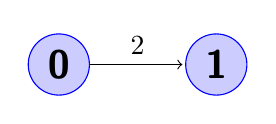
\begin{tikzpicture}[shorten >=1pt, auto, node distance=2cm]
                    \begin{scope}[every node/.style={circle,draw=blue,fill=blue!20!,font=\sffamily\Large\bfseries}]
                    \node (0) {0};
                    \node (1) [right of=0] {1};
                    \end{scope}
                    \begin{scope}[every edge/.style={draw=black,ultra thick}]
                    \draw[->] (0) -- node[above] {2} (1);
                    \end{scope}
                \end{tikzpicture}
            \end{minipage}
            \begin{minipage}{\textwidth}
                \centering
                \vspace{0.2cm}
                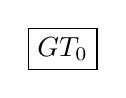
\begin{tikzpicture}[node distance={15mm}, main/.style = {draw, rectangle}] 
                    \node[main] (0) {${GT_{0}}$};
                \end{tikzpicture}
            \end{minipage}
        \end{minipage}
        \begin{minipage}[b]{.5\textwidth}
            \centering
            \begin{minipage}{\textwidth}
                \centering
                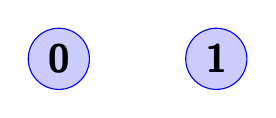
\begin{tikzpicture}[shorten >=1pt, auto, node distance=2cm]
                    \begin{scope}[every node/.style={circle,draw=blue,fill=blue!20!,font=\sffamily\Large\bfseries}]
                    \node (0) {0};
                    \node (1) [right of=0] {1};
                    \end{scope}
                \end{tikzpicture}
            \end{minipage}
            \begin{minipage}{\textwidth}
                \centering
                \vspace{0.2cm}
                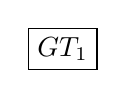
\begin{tikzpicture}[node distance={15mm}, main/.style = {draw, rectangle}] 
                    \node[main] (0) {${GT_{1}}$};
                \end{tikzpicture}
            \end{minipage}
        \end{minipage}
        \begin{minipage}[b]{.5\textwidth}
            \centering
            \begin{minipage}{\textwidth}
                \centering
                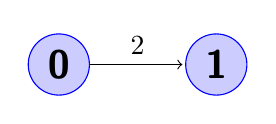
\begin{tikzpicture}[shorten >=1pt, auto, node distance=2cm]
                    \begin{scope}[every node/.style={circle,draw=blue,fill=blue!20!,font=\sffamily\Large\bfseries}]
                    \node (0) {0};
                    \node (1) [right of=0] {1};
                    \end{scope}
                    \begin{scope}[every edge/.style={draw=black,ultra thick}]
                    \draw[->] (0) -- node[above] {2} (1);
                    \end{scope}
                \end{tikzpicture}
            \end{minipage}
            \begin{minipage}{\textwidth}
                \centering
                \vspace{0.2cm}
                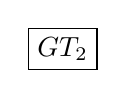
\begin{tikzpicture}[node distance={15mm}, main/.style = {draw, rectangle}] 
                    \node[main] (0) {${GT_{2}}$};
                \end{tikzpicture}
            \end{minipage}
        \end{minipage}
        \begin{minipage}[b]{.5\textwidth}
            \centering
            \begin{minipage}{\textwidth}
                \centering
                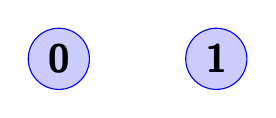
\begin{tikzpicture}[shorten >=1pt, auto, node distance=2cm]
                    \begin{scope}[every node/.style={circle,draw=blue,fill=blue!20!,font=\sffamily\Large\bfseries}]
                    \node (0) {0};
                    \node (1) [right of=0] {1};
                    \end{scope}
                \end{tikzpicture}
            \end{minipage}
            \begin{minipage}{\textwidth}
                \centering
                \vspace{0.2cm}
                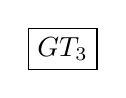
\begin{tikzpicture}[node distance={15mm}, main/.style = {draw, rectangle}] 
                    \node[main] (0) {${GT_{3}}$};
                \end{tikzpicture}
            \end{minipage}
        \end{minipage}
        \begin{minipage}[b]{.5\textwidth}
            \centering
            \begin{minipage}{\textwidth}
                \centering
                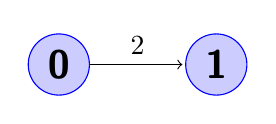
\begin{tikzpicture}[shorten >=1pt, auto, node distance=2cm]
                    \begin{scope}[every node/.style={circle,draw=blue,fill=blue!20!,font=\sffamily\Large\bfseries}]
                    \node (0) {0};
                    \node (1) [right of=0] {1};
                    \end{scope}
                    \begin{scope}[every edge/.style={draw=black,ultra thick}]
                    \draw[->] (0) -- node[above] {2} (1);
                    \end{scope}
                \end{tikzpicture}
            \end{minipage}
            \begin{minipage}{\textwidth}
                \centering
                \vspace{0.2cm}
                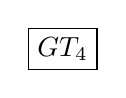
\begin{tikzpicture}[node distance={15mm}, main/.style = {draw, rectangle}] 
                    \node[main] (0) {${GT_{4}}$};
                \end{tikzpicture}
            \end{minipage}
        \end{minipage}
        \begin{minipage}[b]{.5\textwidth}
            \centering
            \begin{minipage}{\textwidth}
                \centering
                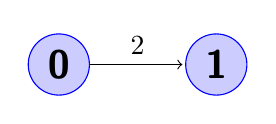
\begin{tikzpicture}[shorten >=1pt, auto, node distance=2cm]
                    \begin{scope}[every node/.style={circle,draw=blue,fill=blue!20!,font=\sffamily\Large\bfseries}]
                    \node (0) {0};
                    \node (1) [right of=0] {1};
                    \end{scope}
                    \begin{scope}[every edge/.style={draw=black,ultra thick}]
                    \draw[->] (0) -- node[above] {2} (1);
                    \end{scope}
                \end{tikzpicture}
            \end{minipage}
            \begin{minipage}{\textwidth}
                \centering
                \vspace{0.2cm}
                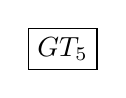
\begin{tikzpicture}[node distance={15mm}, main/.style = {draw, rectangle}] 
                    \node[main] (0) {${GT_{5}}$};
                \end{tikzpicture}
            \end{minipage}
        \end{minipage}
    \end{figure}
\end{figure}

\subsubsection{Algorithme de calcul de la mesure}

\subsubsection{Optimisations faites}

L'algorithme de Dijkstra est donc mis en place et adapté pour les graphes temporels, mais il reste encore des optimisations à faire.
En effet, l'algorithme de Dijkstra est souvent utilisé pour calculer le plus court chemin entre deux noeuds, mais il calcule en réalité beaucoup plus de plus courts chemins.
Donc nous avons modifié l'algorithme pour qu'il écrive directement dans la matrice de distances, puis le but va être d'écrire le plus de distances possibles en une seule fois.

\subsubsubsection{Calcul de la distance entre le noeud de départ et tous les autres noeuds}
Pour connaître la distance entre le noeud de départ et le noeud d'arrivée, Dijkstra va explorer beaucoup de noeuds candidats.
Donc, pour chaque noeud candidat à une distance $d$ du noeud de départ qu'il sort du tas, on va noter cette distance dans la matrice de distances.

\subsubsubsection{Prise en compte de tous les sous-chemins}

Soit un chemin calculé 0->1->2->3, on a un chemin trivial à noter entre 0 et 3, mais on a aussi beaucoup de sous-chemins qui sont calculés.
Ici, on a les chemins 0->1->2, 1->2->3, 0->1, 1->2, 2->3.
Et en général, pour un chemin de taille $n$, on a $n(n-1)/2$ sous-chemins qu'on peut noter dans la matrice de distances.

Nous avons donc créer une structure de données qui va permettre de rapidement stocker tous les sous-chemins à partir des pas faits dans le chemin.
Cette structure ressemble à un arbre de segments, mais en structure pyramidale.
Pour l'exemple précédent, notre pyramide ressemblerait à ça :
0->3
0->1, 1->3
0->1, 1->2, 2->3
\todo{Faire un dessin de la pyramide}

Les éléments 0->1, 1->2, 2->3 sont les briques de la pyramide, qui sont l'équivalent des feuilles de l'arbre de segments.
Dans notre pyramide, chaque élément va stocker le noeud de départ, le noeud d'arrivée, la distance entre ces deux noeuds, et le temps nécessaire pour arriver au noeud de départ.
Ensuite, pour chaque étage de la pyramide, on va regarder notre fils gauche et notre fils droit, ainsi que notre petit-fils commun.
Le noeud de départ sera celui du fils gauche, le noeud d'arrivée celui du fils droit, la distance sera la somme des distances des deux fils moins la distance du petit-fils (partie commune comptée deux fois sinon), et le temps nécessaire pour arriver au noeud de départ sera celui du fils gauche.
S'il n'y a pas de petit-fils, alors la distance commune entre les 2 est comptée.

En les propageant de bas en haut, on va noter tous les sous-chemins possibles dans la matrice de distances, et donc éviter de les recalculer plus tard.

\subsubsubsection{Prédiction des chemins avec le plus d'étapes}

Cette optimisation va de pair avec la précédente, en faisant des benchmarks, nous avons remarqué que parcourir la boucle j à l'envers permettait de gagner du temps.
On suppose que c'est dû au fait que les noeuds avec des indices éloignés soient aussi éloignés dans le graphe,
donc que le chemin entre ces deux noeuds ai plus d'étapes, et que donc on va écrire plus de sous-chemins dans la matrice de distances qui seraint écrasés plus tard si on avait parcouru la boucle dans le sens normal.

\subsubsubsection{Regarder ses voisins}

La distance de $u$ à $v$ est le minimum entre la distance de $u$ à $k$ plus la distance de $k$ à $v$ pour chaque noeud $k$ tel que l'arête $u -> k$ et l'arête $k -> v$ existent.
Donc si nous connaissons toutes ces distances $u -> k$, alors nous pouvons calculer la distance $u -> v$ sans avoir besoin de reparcourir le graphe.

Nous avons utilisé cette propriété pour optimiser notre algorithme.
Tout d'abord, nous créons le graphe inverse, qui pour chaque arête $u -> v$ du graphe original va créer une arête $v -> u$.

Ensuite, pour avoir la distance entre $u$ et $v$, nous cherchons tous les noeuds $k$ tels que l'arête $k -> v$ existe grâce au graphe inverse.
Pour chaque noeud $k$, si la distance est calculée, alors nous pouvons directement la récupérer, sinon nous la calculons.
Ensuite, nous prenons le minimum de toutes ces distances ($u -> k$ + $k -> v$) pour avoir la distance $u -> v$.
C'est très utile pour les noeuds qu'on ne peut atteindre que par un seul autre noeud, car ça évite de refaire un parcours avec juste un noeud en plus.

\subsubsubsection{Se rapporter à un parcours de graphe classique quand c'est possible}
\todo{Attaques statiques}

\subsubsubsection{Calcul du non-attqué}
\todo{blehhhhhh}

\todo{est ce que je parle du cache et de la edges map ?}

\subsubsection{Complexité de l'algorithme}

Donc même si la compléxité pire cas de faire des Dijkstra pour chaque noeud est en $O(n^3 \log n * t)$, la complexité amortie est bien meilleure.
La calculer réellement serait extrêmement complexe et dépend beaucoup de la topologie du graphe, mais sur des villes réelles, nous avons mesurer l'évolution du temps de calcul en fonction du nombre de noeuds, et nous avons obtenu cette courbe :
\todo{Courbe de la complexité}
qui peut être modélisée par une fonction en $O(???????)$.

\todo{Calcul de la mesure}